 \begin{frame}
  \frametitle{architecture Altarica}
  \center
  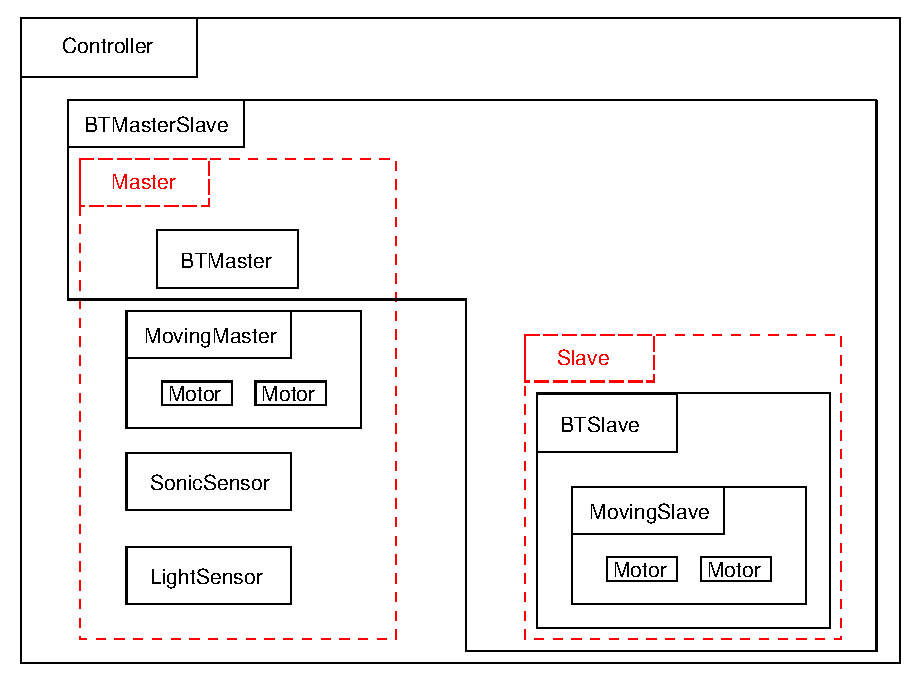
\includegraphics[width=10cm]{ARmodel.eps}

 \end{frame}
 
 
 \begin{frame}
  \frametitle{Le noeud LightSensor}

    \begin{block}{2ème version du noeud}
    \verbatiminput{../src/altarica/alt/LightSensor.alt}
    \end{block}
    
    \begin{block}
    \begin{itemize}
      \item Au début, variable d'état
	  \uncover<2->{
      \item Mais l'environnement est incontrôlable}
	  \uncover<3->{
      \item donc utilisation d'une variable de flux}
	  \uncover<4->{
      \item trois seuils de couleur à détecter}
   \end{itemize}
  \end{block}

 \end{frame}
 
  \begin{frame}
  \frametitle{Le noeud Moving master}

    \begin{block}
    \verbatiminput{../src/altarica/alt/MovingMaster.alt}
    \end{block}
    
    \begin{block}
    \begin{itemize}
      \item Au début, variable d'état
	  \uncover<2->{
      \item Mais l'environnement est incontrôlable}
	  \uncover<3->{
      \item donc utilisation d'une variable de flux}
	  \uncover<4->{
      \item trois seuils de couleur à détecter}
   \end{itemize}
  \end{block}

 \end{frame}
